\documentclass{article}

\usepackage{amsmath, amsthm, amssymb, latexsym, amsfonts}
\usepackage{comment, enumerate, mathrsfs, stmaryrd, hyperref}
\usepackage{tikz}
\usepackage{xcolor}
\usepackage{listings}
\usepackage{graphicx}
\usepackage{titlesec}
\usepackage{booktabs}
\usepackage{graphicx}
\usepackage{tabularx}
\usepackage{blindtext}
\usepackage[a4paper, total={7in, 9in}]{geometry}
\usepackage[toc,page]{appendix}

\definecolor{codegray}{gray}{0.9}
\newcommand{\code}[1]{\colorbox{codegray}{\texttt{#1}}}

\definecolor{codegreen}{rgb}{0,0.6,0}
\definecolor{codepurple}{rgb}{0.58,0,0.82}
\definecolor{backcolour}{rgb}{0.95,0.95,0.92}

\lstdefinestyle{mystyle}{
    backgroundcolor=\color{backcolour},   
    commentstyle=\color{codegreen},
    keywordstyle=\color{magenta},
    numberstyle=\tiny\color{codegray},
    stringstyle=\color{codepurple},
    basicstyle=\ttfamily\footnotesize,
    breakatwhitespace=false,         
    breaklines=true,                 
    captionpos=b,                    
    keepspaces=true,                 
    numbers=left,                    
    numbersep=5pt,                  
    showspaces=false,                
    showstringspaces=false,
    showtabs=false,                  
    tabsize=2
}

\lstset{style=mystyle}

\begin{document}

\begin{titlepage}
    \begin{center}
        \vspace*{0.6cm}
            
        \Huge
        \textbf{Do you like Texas hold 'em}
            
        \vspace{0.5cm}
        \LARGE
        STAT230 Real World Assignment 2024W
            
        \vspace{1.5cm}
            
        \textbf{Eason Li, Johnson Ji}
            
        \vspace{3.6cm}
        
        \begin{center}
            
\includegraphics[width = 0.4\textwidth]{images/UofLoo.png}
        \end{center}

        \vspace{0.4cm}
            
        \Large
        Falculty of Math \\
        University of Waterloo \\
        Canada \\
        April 8, 2024
    \end{center}
\end{titlepage}

\newpage

\begin{center}
    \textcolor{blue}{
        In this report, we consider the case a player uses the best 
        five-card poker hand out of seven cards.
    }
\end{center}



\section*{Starting Hands (with 2 players)}

Out of the $\displaystyle \binom{52}{2}$ possible starting hands, there 
are $13 \times 13$ distinct types of starting hands since there are 13 
ranks, there are 13 distinct pocket pairs (e.g. AA), $\displaystyle 
\binom{13}{2} = 78$ distinct suited 2-card combinations (e.g. AKs) 
and $\displaystyle \binom{13}{2} = 78$ distinct unsuited 2-card 
combinations (e.g. AKo). Notice that 
\[
    13 \times 13 = 13 + \binom{13}{2} + \binom{13}{2}
\]
It is intended to calculate the pre-flop 
(before any community cards are dealt) win rate for each distinct 
2-card combination. For each distinct combination, there are 
\[
    \left[ \; \prod_{i = 1}^{n - 1} \binom{52 - 2i}{2} \; \right] \times \binom{52 - 2n}{5}
\] 
possible outcomes for n players. A simulation (Appendix) 
size of $100 \; 000$ is chosen for this section:
\begin{align*}
    & \code{Pocket Pair: 5976} \\
    & \code{Suited: 23167} \\
    & \code{Unsuited: 70857} \\
    & \code{Contains Ace or King: 28643} \\
    & \code{Does Not Contain Ace or King: 71357}
\end{align*}
Recall that we consider in a game consisting two players. In theory, we 
know that the probability of getting pocket pair in a deck of 52 cards is
\[
    \frac{52}{52} \cdot \frac{3}{51} \approx \boxed{0.058823}
\]
the probability for suited pair is 
\[
    \frac{52}{52} \cdot \frac{12}{51} \approx \boxed{0.235294}
\]
while the probability for unsuited pair is 
\[
    \frac{52}{52} \cdot \frac{39}{51} - \frac{52}{52} \cdot \frac{3}{51} 
    \approx \boxed{0.707014}
\]
Lmao our simulations are pretty close to our theoretical values. 




\section*{Poker Hands}

The chance of making, winning and tying with each poker hand is 
investigated. The total number of possible outcomes for a hand 
of poker between $n$ players is given by:
\[
    \left[ \; \prod_{i = 0}^{n - 1} \binom{52 - 2i}{2} \; \right] \cdot \binom{52 - 2n}{2}
\]
which is $2.781 \times 10^{12}$ for just 2 players. 
Since it isn't realistic to go through all possible outcomes,
a simulation (Appendix) size of $100 \; 000$ is chosen (with 2 players):
\begin{align*}
    \begin{split}
        Player \; 1: \\
        \code{Straight Flush: 4} \\
        \code{Quad: 15} \\
        \code{Full House: 250} \\
        \code{Flush: 307} \\
        \code{Straight: 447} \\
        \code{Triple: 536} \\
        \code{Two Pairs: 2341} \\
        \code{Pair: 4355} \\
        \code{High Card: 1745} 
    \end{split}
    \quad
    \begin{split}
        & Player \; 2: \\
        & \code{Straight Flush: 5} \\
        & \code{Quad: 11} \\
        & \code{Full House: 259} \\
        & \code{Flush: 274} \\
        & \code{Straight: 439} \\
        & \code{Triple: 461} \\
        & \code{Two Pairs: 2368} \\
        & \code{Pair: 4395} \\
        & \code{High Card: 1788} 
    \end{split}
\end{align*}
We can also calculate the theoretical expression of the 
absolute frequency of the occurences of each hands:
\begin{enumerate}
    \item \textbf{Straight flush (including royal straight flush):}
    \[
        \binom{10}{1} \binom{4}{1} \binom{46}{2} 
        = 4,324
    \]
    \item \textbf{Quad:} 
    \[
        \binom{13}{1} \binom{48}{3} 
        = 224,848
    \]
    \item \textbf{Full house:}
    \[
        \left[ \binom{13}{2} \binom{4}{3}^2 \binom{44}{1} \right]
        + \left[ \binom{13}{1} \binom{12}{2} \binom{4}{3} \binom{4}{2}^2 \right]
        + \left[ \binom{13}{1} \binom{12}{1} \binom{11}{2} \binom{4}{3} \binom{4}{2} \binom{4}{1}^2 \right]
        \approx 3,473,184
    \]
    \item \textbf{Flush:}
    \[
        \left[ \binom{4}{1} \times \left[ \binom{13}{7} - 217 \right] \right]
        + \left[ \binom{4}{1} \times \left[ \binom{13}{6} - 71 \right] \times 39 \right]
        + \left[ \binom{4}{1} \times \left[ \binom{13}{5} - 10 \right] \times \binom{39}{2} \right]
        \approx 4,047,644
    \]
    \item \textbf{Straight:}
    \[
        [217 \times [4^7 - 756 - 4 - 84]] 
        + [71 \times 36 \times 990] 
        + \left[ 10 \times 5 \times 4 \times [256 - 3] + 10 \times \binom{5}{2} \times 2268 \right]
        \approx 6,180,020
    \]
    \item \textbf{Triple:}
    \[
        \left[ \binom{13}{5} - 10 \right] \binom{5}{1} \binom{4}{1} \left[ \binom{4}{1}^4 - 3 \right]
        \approx 6,461,620
    \]
    \item \textbf{Two pair:}
    \[
        [1277 \times 10 \times [6 \times 62 + 24 \times 63 + 6 \times 64]]
        + \left[ \binom{13}{3} \binom{4}{2}^3 \binom{40}{1} \right]
        \approx 31,433,400
    \]
    \item \textbf{One pair:}
    \[
        \left[ \binom{13}{6} - 71 \right] \times 6 \times 6 \times 990
        \approx 58,627,800
    \]
    \item \textbf{High cards:}
    \[
        1499 \times [ 4^7 - 756 - 4 - 84 ]
        \approx 23,294,460
    \]
\end{enumerate}
Therefore, since we know that the total number of possible combination 
of 7 cards is $\displaystyle \binom{52}{7} = 133,784,560$, hence we can 
find the probability of each hand:
\begin{table*}[ht]
    \centering
    \begin{tabular}{p{0.4\linewidth} | p{0.4\linewidth}}
    \hline
    Poker Hands & Probability \\
    \hline 
    \\
    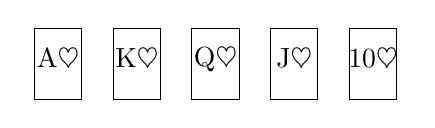
\begin{tikzpicture}
        \foreach \rank/\suit/\x in {A/\(\heartsuit\)/0, K/\(\heartsuit\)/1, Q/\(\heartsuit\)/2, J/\(\heartsuit\)/3, 10/\(\heartsuit\)/4} {
        % Draw the card
        \draw (\x,0) rectangle ++(0.6,0.9);
        % Add the rank and suit
        \node at (\x+0.3,0.5) {\rank\suit};
        }
    \end{tikzpicture} Strait Flush & \qquad \qquad \( \displaystyle \frac{4,324}{133,784,560} \approx 0.0311\% \) \\
    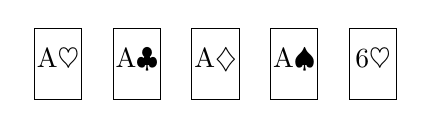
\begin{tikzpicture}
        \foreach \rank/\suit/\x in {A/\(\heartsuit\)/0, A/\(\clubsuit\)/1, A/\(\diamondsuit\)/2, A/\(\spadesuit\)/3, 6/\(\heartsuit\)/4} {
        % Draw the card
        \draw (\x,0) rectangle ++(0.6,0.9);
        % Add the rank and suit
        \node at (\x+0.3,0.5) {\rank\suit};
        }
    \end{tikzpicture} Quad & \qquad \qquad \( \displaystyle \frac{224,848}{133,784,560} \approx 0.168\% \) \\
    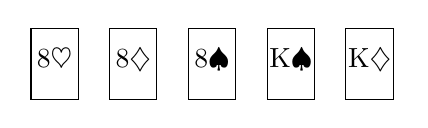
\begin{tikzpicture}
        \foreach \rank/\suit/\x in {8/\(\heartsuit\)/0, 8/\(\diamondsuit\)/1, 8/\(\spadesuit\)/2, K/\(\spadesuit\)/3, K/\(\diamondsuit\)/4} {
        % Draw the card
        \draw (\x,0) rectangle ++(0.6,0.9);
        % Add the rank and suit
        \node at (\x+0.3,0.5) {\rank\suit};
        }
    \end{tikzpicture} Full House & \qquad \qquad \( \displaystyle \frac{3,473,184}{133,784,560} \approx 2.60\% \) \\
    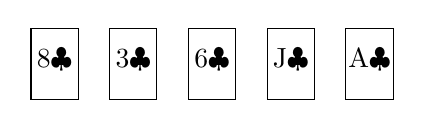
\begin{tikzpicture}
        \foreach \rank/\suit/\x in {8/\(\clubsuit\)/0, 3/\(\clubsuit\)/1, 6/\(\clubsuit\)/2, J/\(\clubsuit\)/3, A/\(\clubsuit\)/4} {
        % Draw the card
        \draw (\x,0) rectangle ++(0.6,0.9);
        % Add the rank and suit
        \node at (\x+0.3,0.5) {\rank\suit};
        }
    \end{tikzpicture} Flush & \qquad \qquad \( \displaystyle \frac{4,047,644}{133,784,560} \approx 3.03\% \) \\
    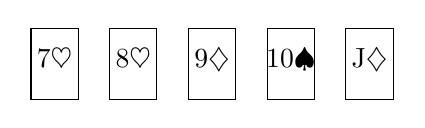
\begin{tikzpicture}
        \foreach \rank/\suit/\x in {7/\(\heartsuit\)/0, 8/\(\heartsuit\)/1, 9/\(\diamondsuit\)/2, 10/\(\spadesuit\)/3, J/\(\diamondsuit\)/4} {
        % Draw the card
        \draw (\x,0) rectangle ++(0.6,0.9);
        % Add the rank and suit
        \node at (\x+0.3,0.5) {\rank\suit};
        }
    \end{tikzpicture} Straight & \qquad \qquad \( \displaystyle \frac{6,180,020}{133,784,560} \approx 4.62\% \) \\ 
    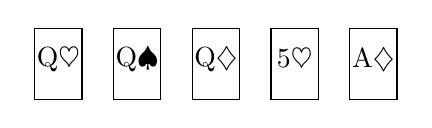
\begin{tikzpicture}
        \foreach \rank/\suit/\x in {Q/\(\heartsuit\)/0, Q/\(\spadesuit\)/1, Q/\(\diamondsuit\)/2, 5/\(\heartsuit\)/3, A/\(\diamondsuit\)/4} {
        % Draw the card
        \draw (\x,0) rectangle ++(0.6,0.9);
        % Add the rank and suit
        \node at (\x+0.3,0.5) {\rank\suit};
        }
    \end{tikzpicture} Triple & \qquad \qquad \( \displaystyle \frac{6,461,620}{133,784,560} \approx 4.83\% \) \\ 
    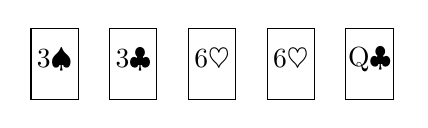
\begin{tikzpicture}
        \foreach \rank/\suit/\x in {3/\(\spadesuit\)/0, 3/\(\clubsuit\)/1, 6/\(\heartsuit\)/2, 6/\(\heartsuit\)/3, Q/\(\clubsuit\)/4} {
        % Draw the card
        \draw (\x,0) rectangle ++(0.6,0.9);
        % Add the rank and suit
        \node at (\x+0.3,0.5) {\rank\suit};
        }
    \end{tikzpicture} Two pairs & \qquad \qquad \( \displaystyle \frac{31,433,400}{133,784,560} \approx 23.5\% \) \\
    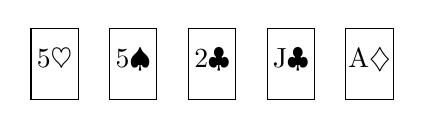
\begin{tikzpicture}
        \foreach \rank/\suit/\x in {5/\(\heartsuit\)/0, 5/\(\spadesuit\)/1, 2/\(\clubsuit\)/2, J/\(\clubsuit\)/3, A/\(\diamondsuit\)/4} {
        % Draw the card
        \draw (\x,0) rectangle ++(0.6,0.9);
        % Add the rank and suit
        \node at (\x+0.3,0.5) {\rank\suit};
        }
    \end{tikzpicture} One pair & \qquad \qquad \( \displaystyle \frac{58,627,800}{133,784,560} \approx 43.8\% \) \\ 
    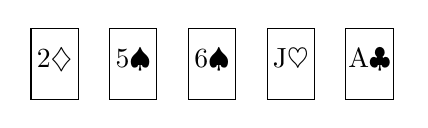
\begin{tikzpicture}
        \foreach \rank/\suit/\x in {2/\(\diamondsuit\)/0, 5/\(\spadesuit\)/1, 6/\(\spadesuit\)/2, J/\(\heartsuit\)/3, A/\(\clubsuit\)/4} {
        % Draw the card
        \draw (\x,0) rectangle ++(0.6,0.9);
        % Add the rank and suit
        \node at (\x+0.3,0.5) {\rank\suit};
        }
    \end{tikzpicture} High hands & \qquad \qquad \( \displaystyle \frac{23,294,460}{133,784,560} \approx 17.4\% \) \\
    \hline
    \end{tabular}
\end{table*}

We can easily discover that all the probabilities sum up to be 1, thus 
we can that this is in fact a multinomial distribution. 




\newpage
\section*{How many times does each player win in a 2-player poker game}

We can also simulate how many times each player wins:

\begin{center}
    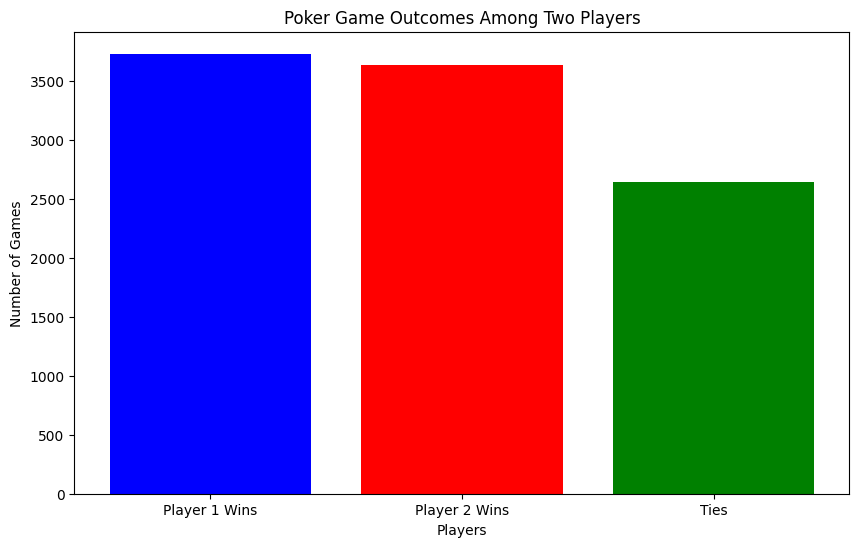
\includegraphics[width = 0.8\textwidth]{images/win_rate_2_player.png}
\end{center}

The bar chart presents the outcomes of poker games between two players. 
It shows the frequency of wins for Player 1, Player 2, and the number 
of games that ended in a tie. Statistically, we can observe that each 
no player has a significant advantage over the other. The small difference 
in the heights of the bars for Player 1 Wins and Player 2 Wins implies 
a roughly uniform distribution of outcomes between the two players. 

Moreover, in a game of 4 player, the winning rates are still fairly close 
among all participants:

\begin{center}
    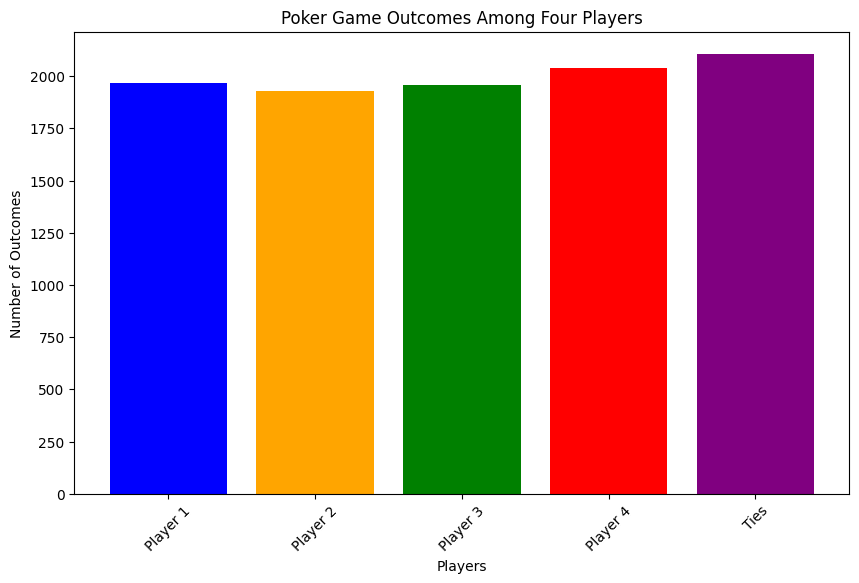
\includegraphics[width = 0.8\textwidth]{images/win_rate_4_player.png}
\end{center}



\section*{Out Odds}
An out in a poker hand can be loosely defined as any card in the deck that will improve your current hand more than your opponents. Probability regarding outs is especially important in actual poker play, as they are a large influential factor regarding your chances of winning the pot. For instance, suppose that you had the following hand:
\begin{center}
    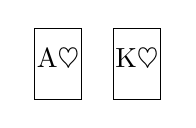
\begin{tikzpicture}
            \foreach \rank/\suit/\x in {A/\(\heartsuit\)/0, K/\(\heartsuit\)/1} {
            % Draw the card
            \draw (\x,0) rectangle ++(0.6,0.9);
            % Add the rank and suit
            \node at (\x+0.3,0.5) {\rank\suit};
            }
        \end{tikzpicture}
\end{center}

And the turn has revealed the following cards:
\begin{center}
    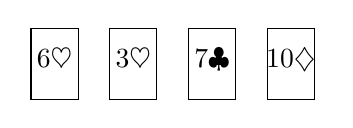
\begin{tikzpicture}
            \foreach \rank/\suit/\x in {6/\(\heartsuit\)/0, 3/\(\heartsuit\)/1, 7/\(\clubsuit\)/2, , 10/\(\diamondsuit\)/3} {
            % Draw the card
            \draw (\x,0) rectangle ++(0.6,0.9);
            % Add the rank and suit
            \node at (\x+0.3,0.5) {\rank\suit};
            }
        \end{tikzpicture}
\end{center}

In this situation, your outs on the river are if any heart is revealed 
($13-4 = 9$ possibilities) to form a flush, or if any ace or king is 
revealed ($3+3 = 6$ possibilities) to form top pair. Summing these 
together, we obtain that our total number of outs is $15$, and our 
out odds are $15/(52-6) \approx 32.6\%$.

\section*{Expected Value of Calling}

Continuing this example, suppose that the current pot has \$50, and our 
opponent has just raised by \$30. We can calculate the expected value 
of calling, and use this to determine whether a call is profitable or 
not. By using our out odds as a rough substitute for our equity, or the 
chance that we win the pot, we can use the formula for expected value: 
\[
    
\]E[X] = P(\text{winning}) \cdot \text{gain} - P(\text{losing}) \cdot \text{loss}$$
So for instance, in this example, our probability of winning would be $32.6\%$, and our probability of losing would be $100\%-32.6\% = 67.4\%$. Our gain would be equal to $\$80$, and our loss would be $\$30$ because we are essentially putting in $\$30$ to have a chance of winning the pot after our opponent has raised. Plugging these values into the formula, we obtain:
$$E[X] = 0.326 \cdot \$80 - 0.674 \cdot \$30 = \$5.83$$
Hence, a call is theoretically profitable. \\

However, this model skips out on many other details associated with the game of poker. For one, this assumes that an out is equivalent to winning the round, which isn't really reasonable. The opponent could have any range of cards that beat your hand, and there really isn't any way to know for certain. Furthermore, there's also the knowledge of knowing how likely your opponent is to bluff. Depending on this factor, it may be ideal to bet on unprofitable calls. But above all, these formulae are ultimately guidelines for you to follow. Statistics can and will help guide you along in times of confusion, but its your intuition that is your strongest weapon, and what will win you the most games.



\newpage
\section*{Appendices}

\subsection*{Some code modelling poker hands:}

\begin{center}
    \begin{lstlisting}[language=Python]
        for _ in range(num_simulations):
            deck = create_deck()
            random.shuffle(deck)
            
            player1_cards = deck[:2]
            player2_cards = deck[2:4]
            community_cards = deck[4:9]
            
            player1_hand = find_best_hand(player1_cards + community_cards)
            player2_hand = find_best_hand(player2_cards + community_cards)
            
            hand_type_counters['Player 1'][player1_hand] += 1
            hand_type_counters['Player 2'][player2_hand] += 1

        for player, counters in hand_type_counters.items():
            print(f"{player}:")
            for hand_type, count in counters.items():
                print(f"{hand_type}: {count}")
            print()
        \end{lstlisting}
\end{center}

This code simulates multiple rounds of a poker game, shuffling and 
distributing a deck of cards between two players and the community 
pool in each round. It eventually prints a summary of how often 
each type of hand occurred for each player, providing insights into 
the distribution of hand types over the simulated games.

\subsection*{Some code modelling winning frequencies in a two-player game:}

\begin{center}
    \begin{lstlisting}[language=Python]
        def simulate_games(num_games):
            player1_wins = 0
            player2_wins = 0
            ties = 0
            
            for _ in range(num_games):
                deck = create_deck()
                player1_hand, player2_hand, community_cards = deal_hands(deck)
                
                result = evaluate_and_compare_hands
                (player1_hand + community_cards, player2_hand + community_cards)
                
                if result == 'player1':
                    player1_wins += 1
                elif result == 'player2':
                    player2_wins += 1
                else:
                    ties += 1
            
            return player1_wins, player2_wins, ties
    \end{lstlisting}
\end{center}

The ``simulate\_games'' function runs a specified number of poker 
games between two players, counting wins for each player and ties.
Wins for each player and ties are tallied and returned at the end, 
providing a summary of game results.







\end{document}
